\begin{figure*}[ht]
\begin{minipage}{.7\textwidth}
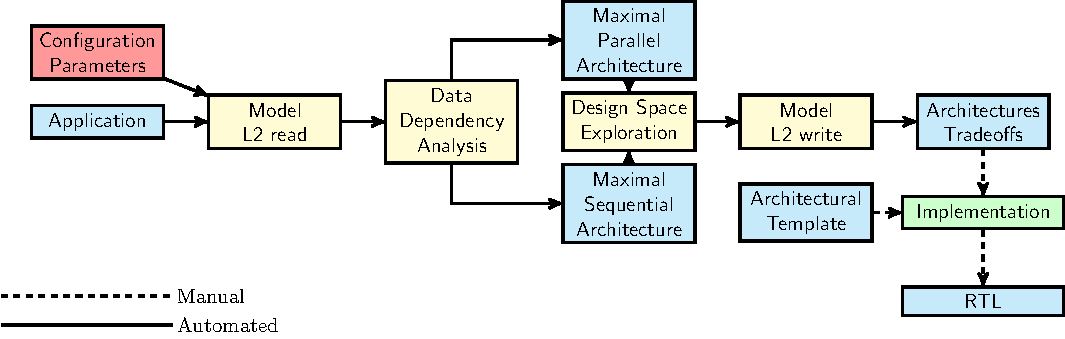
\includegraphics[width=.9\textwidth,left]{images/framework.pdf}
  \caption{\small \frameworkname~Framework.}{}
  \label{fig:framework}
\end{minipage}%
\begin{minipage}{.3\textwidth}
    \centering
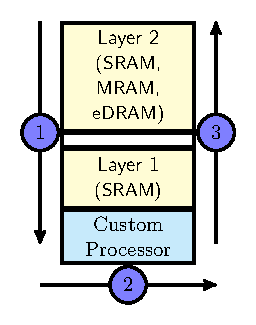
\includegraphics[width=.5\textwidth]{images/architecture.pdf}
\caption{\small The system under analysis. 
    %Composed by two levels of memory, the memory at layer two can use various technologies while the memory at layer one uses only SRAM technology.
    }
\label{fig:system}
\end{minipage}
\end{figure*}
\section{Framework}
\label{sec:framework}
The framework presented in this work allows the user to \textbf{customize} the different building blocks to be used in the design of the custom processor and memory system, \textbf{explore} custom architectures automatically generated for a given application and \textbf{estimate} area, power and latency of each of the architectures. Figure~\ref{fig:framework} gives an overview of the different steps in the framework. The framework takes two inputs, the \textit{Configuration Parameters} - described in Section~\ref{ssec:conf_param} - and an \textit{Application} - detailed in Section~\ref{ssec:app}. A set of hardware architectures, behaviorally equivalent to the input application, is automatically generated by the framwork and the area, power and latency trade-off is generated. The generated hardware architectures can be used to generate an RTL implementation using the \textit{architectural templates} described in Section~\ref{sec:arch_template}.
The framework is composed of three main steps. The first step - \textit{L2 Model} - models the transfer of the input data between the \textit{Level 2} memory and the \textit{Level 1} memory. The second step, \textit{Data Dependency Analysis} performs static analysis on the input application. The last step, \textit{Design Space Exploration}, uses the information extracted by the previous step to procedurally generate different hardware architectures.
The rest of this section will describe more in detail the different inputs and steps of the framework.
%\begin{figure*}[tb] 
%\centering
%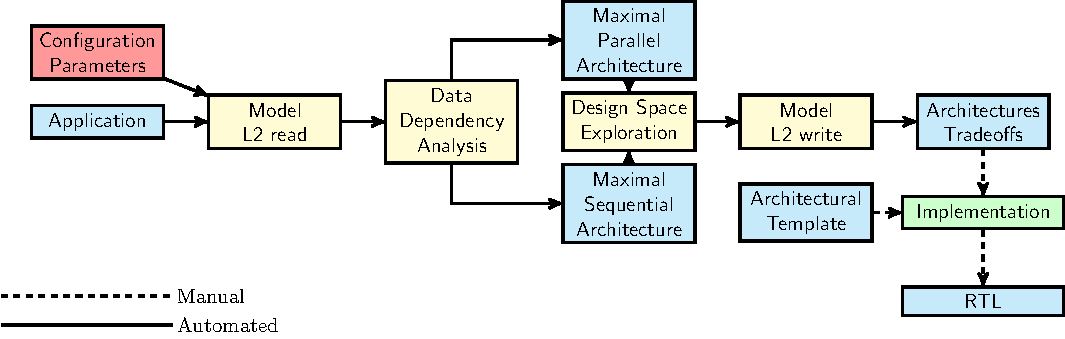
\includegraphics[width=1.5\columnwidth]{images/framework.pdf}
%\caption{\small Diagram of the Framework presented in this work.}
%\label{fig:framework}
%\end{figure*}



%\begin{figure}
%\centering
%\begin{subfigure}{.5\textwidth}
%  \centering
%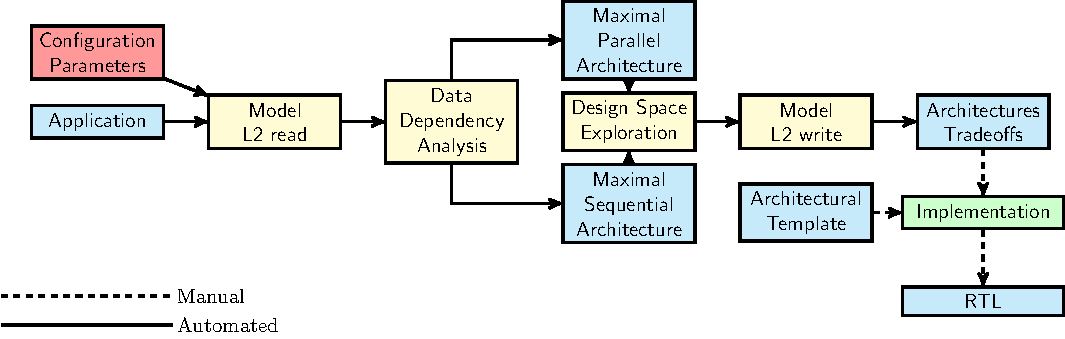
\includegraphics[width=0.4\linewidth]{images/framework.pdf}
%  \captionof{figure}{\small Diagram of the Framework presented in this work.}
%  \label{fig:framework}
%\end{subfigure}%
%\begin{subfigure}{.5\textwidth}
%  \centering
%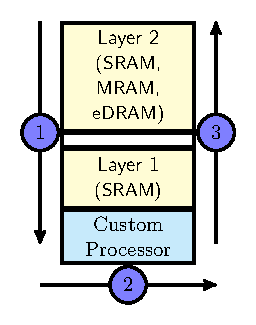
\includegraphics[width=0.3\linewidth]{images/architecture.pdf}
%\captionof{\small The system under analysis. }
%\label{fig:system}
%
%\end{subfigure}
%\caption{A figure with two subfigures}
%\label{fig:test}
%\end{figure}

\subsection{Model of Execution}
\label{ssec:system_under_analysis}
The system architecture we assume in this work is composed of two levels of memory and a custom processor, as shown in Figure~\ref{fig:system}. The first level of memory - \textit{Level 1} - smaller in size and uses SRAM as it needs to be physically close to the processor for faster access. The second layer - \textit{Level 2} - larger in size and can be any memory technology (on-chip or off-chip) with diffferent access latency for read and write operations. Note that the processor and \textit{Level 1} memory runs at a different clock speed than the \textit{Level 2} memory. We assume a model of execution, as illustrated in Figure~\ref{fig:system}, by the three steps. Initially, all of the required input data for one iteration of the application are available at the \textit{Level 2} memory. In the first step, part of the input data is transfered to the custom processor using the \textit{Level 1} memory as intermediate storage location. In the second step, the computation is peformed in the processor and the output elements are stored in the \textit{Level 1} memory. Once the computation is complete, in the third step, the output data stored in the \textit{Level 1} memory is transfered back to the \textit{Level 2} memory. Note that our model of execution performs all the three steps in a pipelined manner.

%Taking advantage of the possibility to produce stacked chip having levels produced using different manufacturing technologies we are able to explore different memory implementations at the \textit{Level 2} of the memory architecture.

%\begin{figure}[tb] 
%\centering
%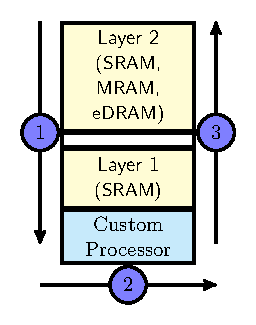
\includegraphics[width=0.25\columnwidth]{images/architecture.pdf}
%\caption{\small The system under analysis. Composed by two levels of memory, the memory at layer two can use various technologies while the memory at layer one uses only SRAM technology.}
%\label{fig:system}
%\end{figure}

\subsection{Level 2 Memory Model}
\label{ssec:layer2_model}
Since the \textit{Level 2} memory has longer access latency, we model them assuming the data is accessed in larger bursts.
%Figure~\ref{fig:l2model}  shows a representation of such access. 
A read or write burst access to the \textit{Level 2} memory is controlled by a Direct Memory Access (DMA) controller, with the starting address and size of the burst given as input to the DMA. After an initial \textit{setup latency}, the accessed elements are transfered in sequence from the start address to the end address, to the \textit{Level 1} memory if a read access is being performed or to the \textit{Level 2} memory for a write access.

\subsection{Application}
\label{ssec:app}
The framework performs exact data dependency analysis on the input application. This entails that the behaviour of the application needs to be completely specified at compile-time and independent from the input data. Streaming applications meet these requirement and can be analyzed by our framework. The input application language that our framework currently supports is C/C++, however the framework uses the LLVM Intermediate Representation~\cite{llvm}, so it can easily be extended to support other languages as well.
%\begin{lstlisting}[language=C, caption={Example of input application, C implementation of a matrix vector multiplication.}, label={lst:matrixvec}]
%void matrix_vec_kernel(int *A,int *B, int *C){
%    int sum;
%    for(int i=0;i<DIM2;i++){
%        sum=0;
%        for(int j=0;j<DIM1;j++){
%            sum+=A[i*DIM1+j]*B[j];
%        }
%        C[i]=sum;
%    }
%}
%\end{lstlisting}

\subsection{Configuration Parameters}
\label{ssec:conf_param}
The second input to the framework is a configuration file that contains description of the different building blocks to be used in the realization of the hardware architecture. Through this file, the user can specify - different compute units - e.g. multipliers, adders, - process technology to be used - e.g. 16nm, 28nm - the clock frequency of processor \& Level 1 memory and Level 2 memory. Moreover, the user can specify the datawidth used by the compute units and the Level 1 and Level 2 memories. 
Information requred to model the Level 2 burst accesses are as well specified in this file: the setup latency for write/read accesses, the type of Level 2 memory to be used -e.g. MRAM, SRAM etc..- and the size of the Level 2 memory. The different parameters in the configuration file are then used to access a database containing estimates (obtained by synthesis or from specs) of area usage, static and dynamic power and latency of each of the building blocks.

%\begin{lstlisting}[language=json, caption={Example of input configuration file}, label={lst:conf_file}]
%{ 
%   "resource_database": { 
%	"technology": 16, 
%	"clock_frequency": 1000, 
%	"bitwidth_adder": 128, 
%	"bitwidth_multiplier": 64, 
%	"bitwidth_register_file": 128, 
%	"type_l2": "tt1v1v85c", 
%	"technology_l2": 16, 
%	"clock_l2": 800, 
%	"bitwidth_l2": 32, 
%	"depth_l2":2048, 
%	"setup_write_latency_l2":2, 
%	"setup_read_latency_l2":2 
%   } 
%}
%
%\end{lstlisting}

\subsection{Level 2 Read}
\label{ssec:l2_read_model}
The first operation performed by the framework is to compute the transfer time of the application's input data from the \textit{Level 2} memory to the \textit{Level 1} memory. An address in Level 2 memory is given to the each input element used by the application; different datastructures are placed in consecutive memory addresses. The entire data transfer is modeled as a single burst read operation to the \textit{Level 2} memory. The information required to compute the arrival clock time of each input element to the Level 1 memory is extracted from teh \textit{Configuration Parameters} and performing static analysis on the input \textit{Application}.
Using this information, the exact clock at which each input elements arrives in the Level 1 memory can be computed as:
$$
AClk_i = SL_r + RL_{L2} * (Add_{L2i}+1) * \frac{B_{L1}}{B_{L2}} * \frac{Clk_{L1}}{Clk_{L2}}
$$

Where $AClk_i$ is the clock at which element i arrives to the Level 1 memory, $SL_r$ is the setup latency of a Level 2 burst read, $RL_{L2}$ is the Level 2 read latency - i.e. latency of a single read operation - expressed in number of \textit{Level 2} clock cycles, $Add_{L2i}$ is the offset of element i from the beginning of the burst access, $B_{L1}$ is the data bitwidth of the Level 1 memory, $B_{L2}$ is the data bitwidth of the Level 2 memory, $Clk_{L1}$ is the clock frequency of the Level 1 memory and $Clk_{L2}$ is the clock speed of the Level 2 memory.

\subsection{Data Dependency Analysis}
The \textit{Data Dependency Analysis} module performs three main operations. First, it extracts \textit{Data Dependency Graph} (DDG) from the application. Then, it schedules the DDG using the As Soon As Possible (ASAP) and As Late As Possible (ALAP) methodologies. Finally, it maps instructions in the DDG to hardware components - or Functional Units (FUs) - using a modified version of the \textit{Interval Partitioning} algorithm~\cite{greedyIntervalPartitioning}.
%This next paragraph might be replaced with a reference
To extract the DDG from an application we use LLVM  and custom transformations. We first convert the input application code to its LLVM Intermediate Representation. We then transform the code into static single assignment (SSA) form and perform full-loop unrolling on all of the application loops. After these transformation there will be no control flow instructions in the application body and each variable will be defined only once. Following the chain of use and definition of the variables is then possible to produce a Data Dependency Graph like the one shown in Figure~\ref{fig:ddg}. 
We further process the obtained DDG in the aim to reduce the length of the path between the input nodes and the output nodes. The reason is that the length of such paths is equivalent to the number of sequential operations required to obtain the outputs which determines the latency of the application. Taking advantage of the associativity of some operation we can transform a long sequence of operations - like the one highlighted in Figure~\ref{fig:ddg} - into an equivalent shorter tree.
%\begin{figure}[ht]
%\begin{minipage}{.5\textwidth}
%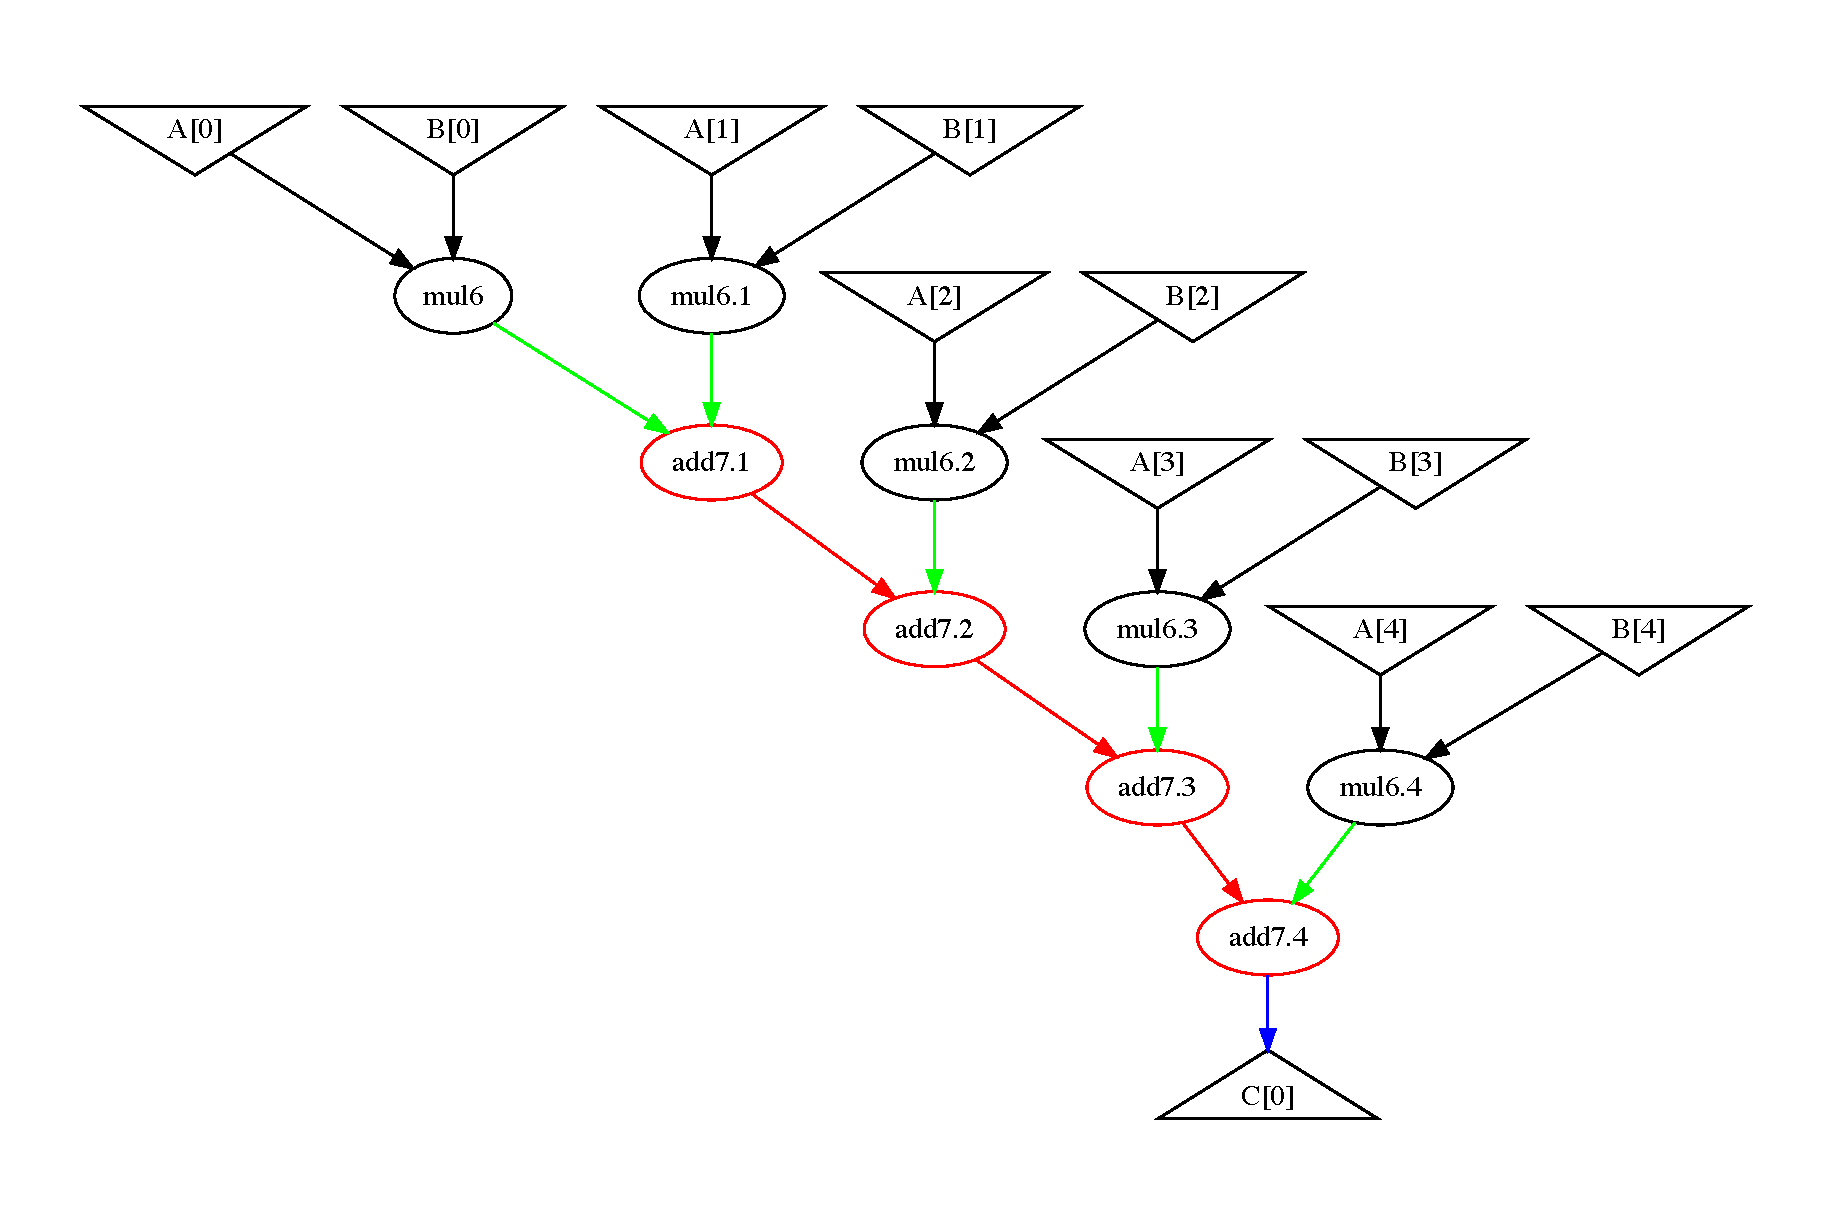
\includegraphics[width=.9\textwidth,left]{images/supernode.pdf}
%  \caption{\small \frameworkname~Framework.}{}
%  \label{fig:framework}
%\end{minipage}%
%\begin{minipage}{.5\textwidth}
%    \centering
%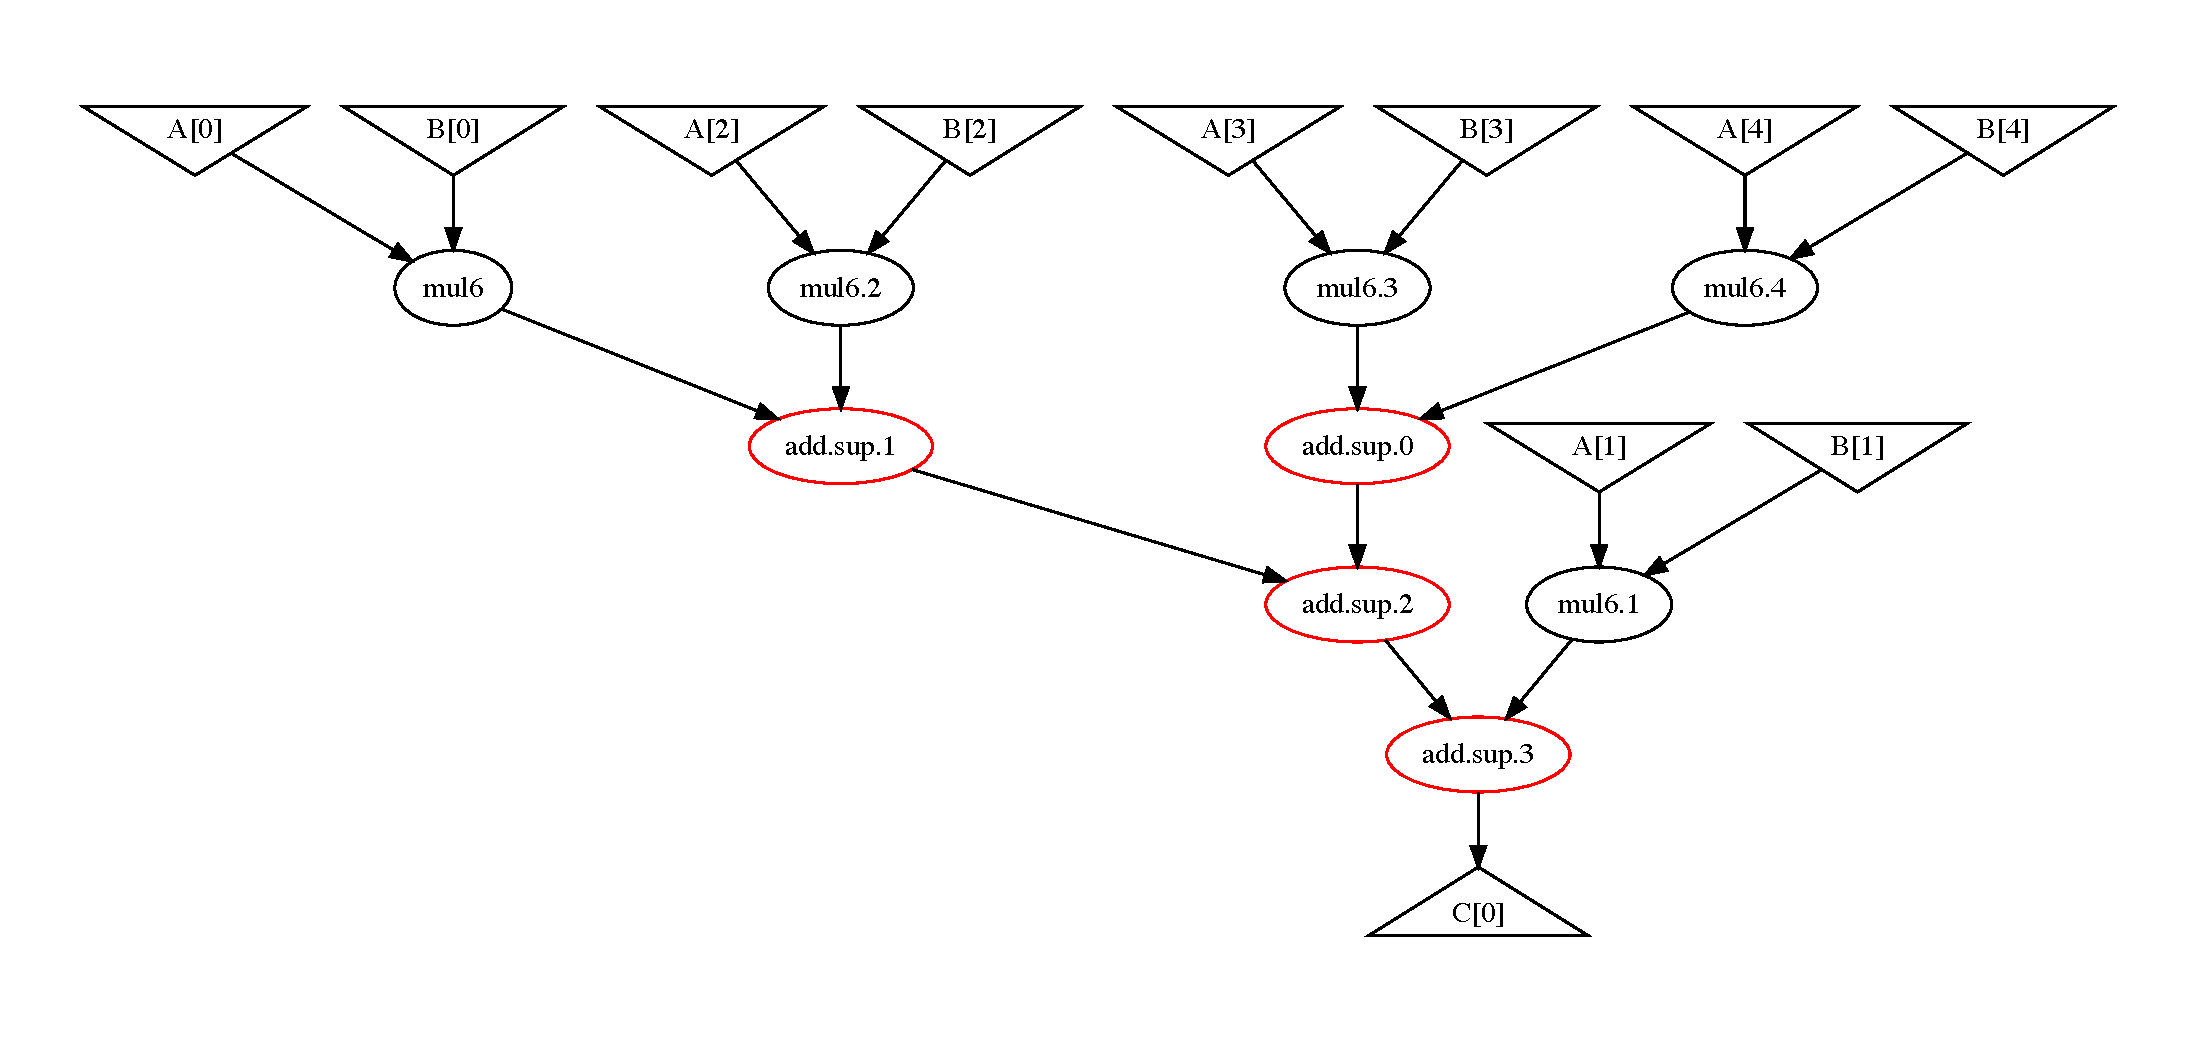
\includegraphics[width=.9\textwidth]{images/supernode_optimized.pdf}
%\caption{\small The system under analysis. 
%    %Composed by two levels of memory, the memory at layer two can use various technologies while the memory at layer one uses only SRAM technology.
%    }
%\label{fig:system}
%\end{minipage}
%\end{figure}

\begin{figure}[tb] 
\centering
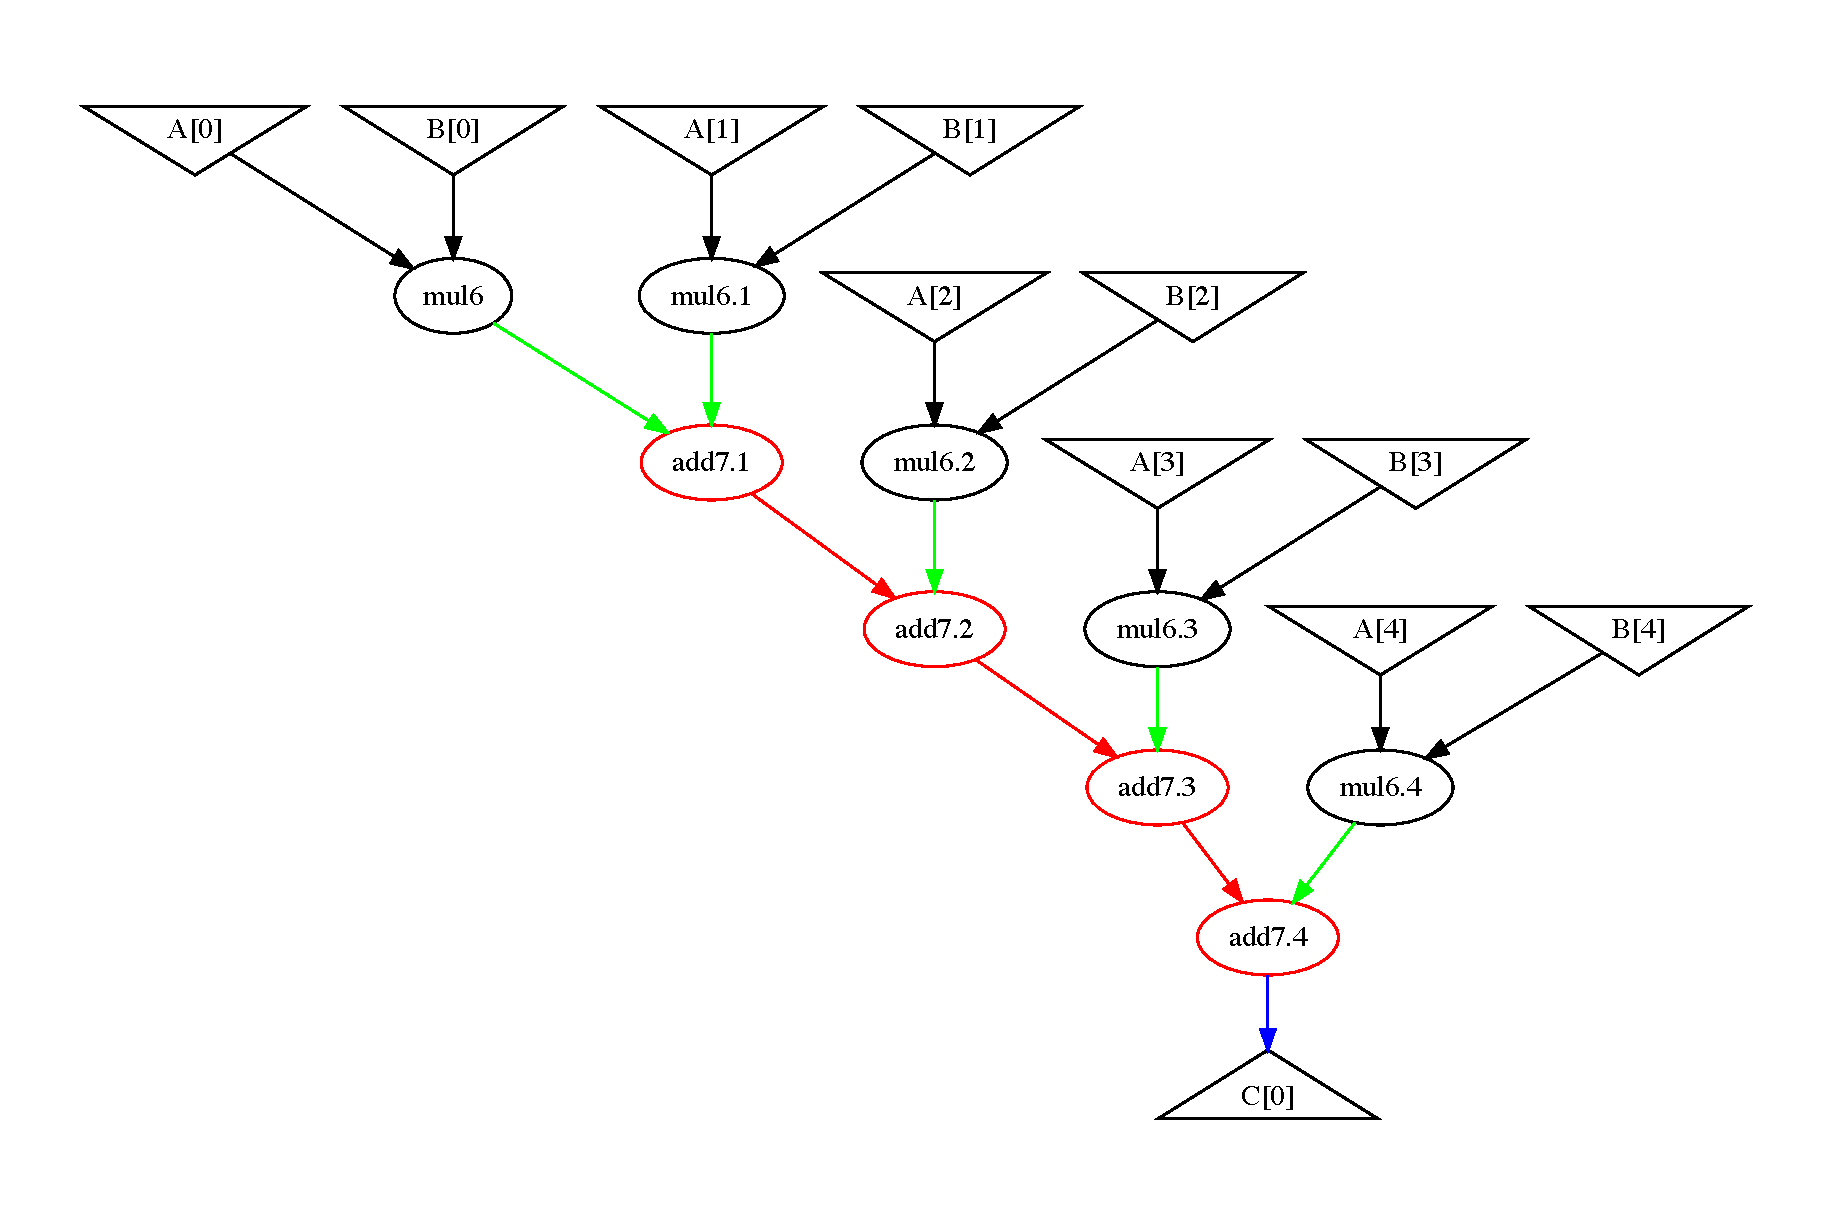
\includegraphics[width=.9\columnwidth,left]{images/supernode.pdf}
    \caption{\small Example of Data Dependency Graph. The inverse triangles represent the input data, obtained from the \textit{load} instructions. The ovals describe operations on data, while the triangle triangle at the bottom represents the result, derived from a \textit{store} instruction.}
\label{fig:ddg}
\end{figure}
%This next paragraph might be replaced with a reference, we are interested mainly in the concept of mobility
In the second step we apply the ASAP and ALAP scheduling methodologies to the generated DDG. These schedules will associate each node of the DDG to a clock cycle where the instruction is executed. We start by scheduling the input nodes of the DDG using the arrival clock time of their element, computed as explained in Section~\ref{ssec:l2_read_model}. This allows us to take into account the transfer time between the Level 2 memory and Level 1 memory. We then derive the minimal latency required to obtain the outputs of the application with the ASAP schedule: starting from the DDG input leafs each instruction node is scheduled as soon as its dependencies are resolved. 
Once a clock is assigned to the output leaf nodes of the DDG we can perform the ALAP scheduling: starting from the output leaf nodes each dependency node is scheduled as late as possible. After this second step, each node will then have an associated ASAP schedule and ALAP schedule. The difference between these two schedules is called \textit{mobility} of the node. The mobility of a node identifies an interval of clocks in which the instruction can be scheduled without changing the overall latency of the application.
The final step of the \textit{Data Dependency Analysis} module - described in Section~\ref{ssec:modified_interval_partitioning} - will allocate the DDG nodes to FU, leveraging the nodes mobility to minimize the number of FUs of the final hardware architecture. 

\subsection{Modified Interval Partitioning}
\label{ssec:modified_interval_partitioning}
To generate an hardware architecture behaviorally equivalent to the input application and with the latency identified during the ASAP-ALAP scheduling, there are two main requirements. The first is that each instruction needs to be computed within its ASAP-ALAP interval. The second requirement is that instructions in the original DDG which are executed by the same FU cannot be scheduled at the same time.
Our Modified Interval Partitioning algorithm - based on the original greedy Interval Partitioning algorithm~\cite{greedyIntervalPartitioning} - is able to generate hardware architectures from a DDG meeting the two requirements described above. The original Interval Partitioning problem addresses the issue of assigning a number of jobs, with known starting and ending time, to the minimum amount of resources ensuring that the jobs assigned to a resource do not overlap. To map the Interval Partitioning formulation to the allocation of instructions to FU, we need to consider application instructions as jobs and FUs as resources. 
There are however three main differences between our problem and the canonical Interval Partitioning. First, while in the original Interval Partitioning problems jobs are equivalent to each other and can be assigned to any resource, the instructions represent computations. For example a multiply instruction can only be assigned to a multiply FU. To address this issue, we divide our initial problem and we perform multiple time the Interval Partitioning, once per operation type. This ensures a correct allocation of the instruction to FUs performing the same operation. The second difference is due to the \textit{mobility} of our instructions. Each instruction does not have a predefined start and end time, like a job has in the original Interval Partitioning, but it has a time interval - derived with ASAP-ALAP - in which it can be scheduled and a fixed latency. Hence, the start time of an instruction might vary, but once this is fixed, its end time can be derived. The modified Interval Partitioning takes the mobility of an instruction into account allowing a given instruction to start at any time within its allowed interval. The last difference regards the dependencies between instructions. While the original jobs in the Interval Partitioning are intependent from each other, the instructions of an application need to be executed according to their dependencies. This is addressed by ensuring that a given instruction is allocated after its dependencies are allocated and by verifying that its starting time is scheduled after the ending time of its dependencies.
Listing~\ref{lst:modified_interval_partitioning} shows the pseudocode of our modified interval partitioning algorithm. 
\begin{lstlisting}[language=Python, caption={Modified Interval Partitioning Algorithm}, label={lst:modified_interval_partitioning}]
FunctionalUnits=[]
sort i in Instructions by ASAP[i]
for each i in Instructions
	allocated = False
	schedule[i] = ASAP[i]
	for d in dep(i)
		end_time_d = schedule[d] + latency(d)
		schedule[i] = max(schedule[i],end_time_d)
	for each fu in FunctionalUnits 
		if type(fu) ==  type(i)
			if ALAP[i] >=  next_free_slot[fu]
				fu += [i]
				schedule[i] = max(schedule[i],
					next_free_slot[fu])
				next_free_slot[fu] = schedule[i] + 
					latency(i)
				allocated = True
	if not allocated
		create new Functional Unit fu
		type(fu) = type(i)
		fu += [i]
		next_free_slot[fu] = schedule[i] + latency(i)
		FunctionalUnits += [fu]

\end{lstlisting}
We assume that ASAP and ALAP schedules have been previously performed, hence we can have two datastructures that return the ASAP and ALAP schedules for a given instruction i - i.e. ASAP[i] and ALAP[i]. Instructions is an ordered list of instructions initialized with the instructions of the input application. A Functional Unit is represented as a set containing the instructions that have been allocated to it, and FunctionalUnits is a set containing the Functional Units of the resulting architecture which is initialized as an empty set. The functions latency and dep take an instruction i as input and return respectively the latency of i and a list of intructions i depends on. The function type
takes as input a Functional Unit or an Instruction and returns the type of operation performed.
The Modified Interval Partitioning algortihms returns the FunctionalUnits and schedule datastructure. FunctionalUnits contains a set of Functional Units which define the generated architecture, each Functional Unit is a set that contains the instrucitons to be executed. The schedule datastructure will contain the clock at which each instruction of the input application has to be executed.

\subsection{Maximum Parallel Architecture and Most Sequential Architecture}
We refer to output hardware architecture obtained after the \textit{Data Dependency Analysis} module as \textbf{Maximum Parallel Architecture}. This architecture will take full advantage of the parallellism of the application and will perform the computation with the minimal possible latency. However, the Maximum Parallel Architecture will use the maximum number of functional units - in the worst case scenario equivalent to the number of instructions in the application - and it will hence have the worst area.
At the other end of the spectrum of architectures we can imagine the \textbf{Most Sequential Architecture}, where no parallelism is used and the instruction are scheduled sequentially respecting their dependencies. This architecture will have the worst possible latency, however the minimal impact in area - using only one Functional Unit per operation type.
Probably none of these two architectures will be of direct interest for the user as they represent two extreme cases. The architecture that are most likely to be interesting are the ones between the Maximum Parallel and Most Sequential that offer tradeoffs between power, latency and area. Section~\ref{ssec:dse} describes how these intermediate architecures can be procedurally generated.

\subsection{Design Space Exploration}
\label{ssec:dse}
The \textit{Design Space Exploration} module procedurally generates hardware architectures, behaviorally equivalent to the input application, which exibit area, latancy and power tradeoffs. 
The DSE performs an iterative process and outputs, at the end of each iteration, a different hardware architecture. The iterative process start from the \textbf{Maximum Parallel Architecture} and ends when the \textbf{Most Sequential Architecture} is generated. 
An iteration consists of three steps. First, the instructions corresponding to output leaf nodes in the DDG are selected. The ALAP schedule of these iterations is increased by 1. After, the ALAP scheduling of the rest of the nodes in the DDG is updated accordingly. Doing so, the mobility of each instruction node is increased by one. The last step of the DSE consists in performing the Modified Interval Partitioning using the new ALAP schedule. Due to the increased mobility of each instruction the generated architecture is likely to use less Functional Unit.
The process stops as soon as one iteration generates the \textbf{Most Sequential Architecture} which can be recognised because it contains only one Functional Unit per operation type.
There are two side benefit of our DSE approach. The first is that it can be tuned. By changing the value that is used to increase the ASAP latency - which is one by default - we can tradeoff the speed of the DSE process for the accuracy. The second benefit is that each iteration is independent from the others hence the DSE process can be easily parallelized.


\subsection{Level 2 Write}
The schedule produced by the Modified Interval Partitioning algorithm already takes into account the transfer of the input data between the Level 2 memory and the Level 1 memory as explained in~\ref{ssec:l2_read_model}. However, it does not include the transfer of the output data from the Level 1 memory to the Level 2 memory - which represents the end of the computation (see~\ref{ssec:system_under_analysis}). But, the result of the scheduling process determines the clock cycle at which the computation is over and the last output is stored in Level 1 memory. The transfer of the outputs to the Level 2 memory can therefore start right after the Custom Processor generates the last output. We model the transfer back to Level 2 as a burst write access, using the formula below we can derive the overall latency.
$$
L2WBL = wSL + L2WL * O * \frac{L2B}{L1B} * \frac{L1Clk}{L2Clk}
$$
Where $L2WBL$ is the Level 2 Write Back Latency, $wSL$ is the setup latency of a Level 2 burst write, $L2WL$ is the Level 2 write latency - i.e. latency of a single write operation - expressed in number of L2 clock cycles, $O$ is the total number of output elements,$L2B$ is the data bitwidth of the Level 2 memory, $L1B$ is the data bitwidth of the Level 1 memory, $L1Clk$ is the clock frequency of the Level 1 memory and $L2Clk$ is the clock speed of the Level 2 memory.

\subsection{Architecture Tradeoffs}
%In section~\ref{
For a given input application and a configuration the framework outputs a set of hardware architectures having different area and latency tradeoffs. Figure~\ref{fig:tradeoffs} show three examples of architecture generated during the DSE. Each box represents a FU; The FUs generated from load and store instructions of the DDG (see Figure~\ref{fig:ddg}) will become separate memory banks of the Level 1 memory. The remaining FU are obtained from operation nodes of the DDG. We allow the architectures to have cycles as the circuit is synchronous and every instruction has been carefully scheduled. A self-loop in a FU idendifies data reuse, section~\ref{sec:arch_template} clarifies how this functionality can be achieved.
\begin{figure}[ht]
\centering
\begin{subfigure}{.4\columnwidth}
  \centering
  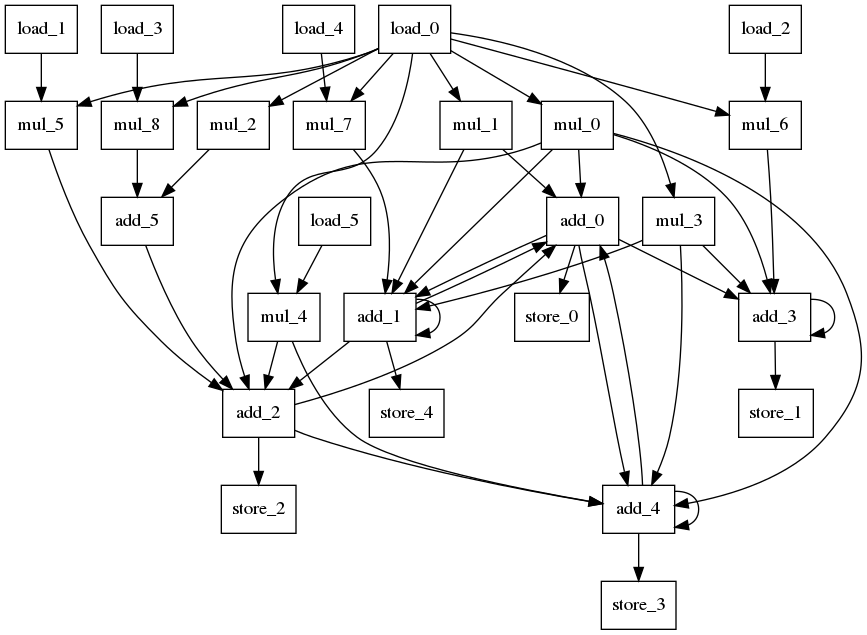
\includegraphics[width=\textwidth]{images/Architecture_latency_146_schematic.png}
  \caption{}
  \label{fig:max_par_arch}
\end{subfigure}%
\begin{subfigure}{.3\columnwidth}
  \centering
  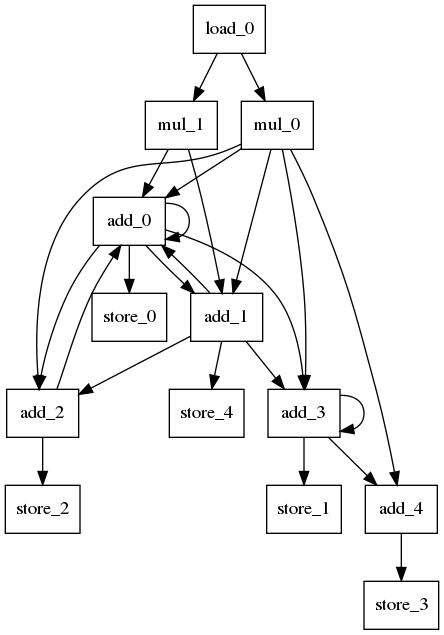
\includegraphics[width=\textwidth]{images/Architecture_latency_166_schematic.png}
  \caption{}
  \label{fig:inter_arch}
\end{subfigure}
\begin{subfigure}{.2\columnwidth}
  \centering
  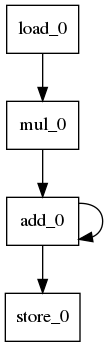
\includegraphics[width=0.5\textwidth]{images/Architecture_latency_188_schematic.png}
  \caption{}
  \label{fig:most_seq_arch}
\end{subfigure}
    \caption{Example of architectures generated from a matrix vector multiply application of size 5x5. The Maximal Parallel Architecture (a), an intermediate architecture (b) and the Most Sequential Architecture (c).}
\label{fig:tradeoffs}
\end{figure}

%\begin{figure}
%
%\begin{minipage}{.5\linewidth}
%\centering
%\subfloat[]{\label{main:a}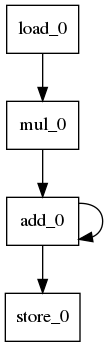
\includegraphics[scale=.2]{images/Architecture_latency_188_schematic.png}}
%\end{minipage}%
%\begin{minipage}{.5\linewidth}
%\centering
%\subfloat[]{\label{main:b}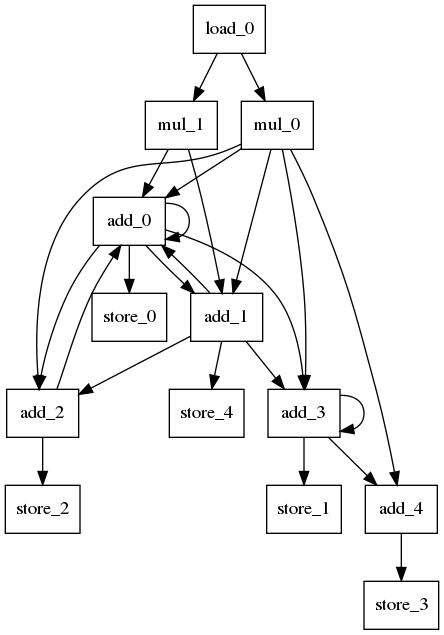
\includegraphics[scale=.2]{images/Architecture_latency_166_schematic.png}}
%\end{minipage}\par\medskip
%\centering
%\subfloat[]{\label{main:c}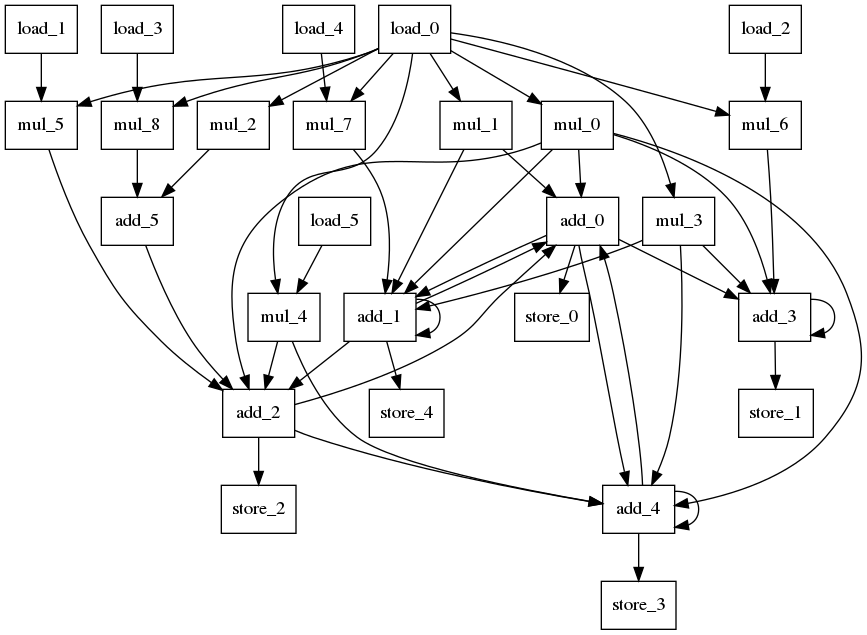
\includegraphics[scale=.10]{images/Architecture_latency_146_schematic.png}}
%
%\caption{my fig}
%\label{fig:main}
%\end{figure}
